\documentclass[12pt]{article}
\textwidth=17cm \oddsidemargin=-0.9cm \evensidemargin=-0.9cm
\textheight=23.7cm \topmargin=-1.7cm

\usepackage{amssymb, amsmath, amsfonts}
\usepackage{moreverb}
\usepackage{graphicx}
\usepackage{enumerate}
\usepackage{graphics}
\usepackage{color}
\usepackage{array}
\usepackage{float}
\usepackage{hyperref}
\usepackage{textcomp}
\usepackage{alltt}
\usepackage{physics}
\usepackage{mathtools}
\usepackage{tikz}
\usetikzlibrary{positioning}
\usetikzlibrary{arrows}
\usepackage{pgfplots}
\usepackage{bigints}
\usepackage[utf8]{inputenc}
\usepackage[english]{babel}
\usepackage{amsthm}
\usepackage{fancyhdr}
\usepackage[makeroom]{cancel}
\pagestyle{fancy}
\allowdisplaybreaks

\newcommand{\E}{\varepsilon}

\newcommand{\suchthat}{\, \mid \,}
\newcommand{\ol}[1]{\overline{#1}}
\newcommand{\bbar}[1]{\overline{#1}}
\newcommand{\inpd}[1]{{\left< \, #1 \, \right>}}
\renewcommand{\theenumi}{\alph{enumi}}
\newcommand\Wider[2][3em]{%
\makebox[\linewidth][c]{%
  \begin{minipage}{\dimexpr\textwidth+#1\relax}
  \raggedright#2
  \end{minipage}%
  }%
}

\def\R{\mathbb{R}}
\def\C{\mathbb{C}}
\def\H{\mathcal{H}}
\DeclareMathOperator*{\esssup}{\text{ess~sup}}
\newcommand{\resolv}[1]{\rho(#1)}
\newcommand{\spec}[1]{\sigma(#1)}
\newcommand{\iffR}{\noindent \underline{$\Longrightarrow$:} }
\newcommand{\iffL}{\noindent \underline{$\Longleftarrow$:} }
\newcommand{\lightning}{\textbf{\Huge \Lightning}}
\newcommand{\spt}[1]{\text{spt}(#1)}
\def\ran{\text{ ran}}
   
\newenvironment{myprob}[1]
    {%before text commands
    %{\Huge \_ \_ \_ \_ \_ \_ \_ \_ \_ \_ \_ \_ \_ \_ \_ \_ \_ \_ } \\
    \noindent{\Huge$\ulcorner$}\textbf{#1.}\begin{em}
    }
    { 
    %after text commands
    \end{em} \\ \hphantom{l} \hfill {\Huge$\lrcorner$} }
%	{\noindent \rule{7.5cm}{2pt} \textgoth{#1} \rule{8.cm}{2pt} \begin{em}}
%	{\end{em}\\ \vspace{0.1pt}\noindent \rule{\textwidth}{2pt}}
%
\setcounter{section}{-1}




\begin{document}
\lhead{MATH228B}
\chead{Carter Johnson - Homework 01}
\rhead{\today}

{\let\newpage\relax} 


%%%%%%%%%%%%%%%%%%%%%%%%%%%%%%%%%%%%%%%%%%%%%%%%%%%%% P1
\begin{myprob}{Problem 1}
Consider the advection equation
$$u_t + au_x = 0 $$
on the interval [0,1) with periodic boundary conditions. Space is discretized as $x_j = j \Delta x$ for $j=0, \dots, N-1,$ so that $\Delta x = 1/N$.  Discretize the spatial derivative with the second-order centered difference operator.
\end{myprob}
\begin{enumerate}[(a)]
\item For simplicity, assume $N$ is odd.  The eigenvectors of the centered difference operator are 
$$v_j^k = \exp(2\pi i k x_j),$$
for $k=-(N-1)/2, \dots, (N-1)/2$.  Compute the eigenvalues. \\

$\implies$ With centered difference operator
  $$D u_j = \dfrac{u_{j+1} - u_{j-1}}{2\Delta x},$$
  we have that 
  \begin{align*}
  D v_j^k &= \lambda_k v_j^k \\
  \dfrac{v^k_{j+1}- v^k_{j-1}}{2\Delta X} &= \lambda_k v_j^k\\
  \dfrac{e^{2\pi i k (x_j+\Delta x)}- e^{2 \pi i k (x_j - \Delta x)}}{2\Delta x} &= \lambda_k v_j^k \\
 \qty( \dfrac{e^{2\pi i k \Delta x}- e^{-2 \pi i k \Delta x}}{2\Delta x }) v_j^k &= \lambda_k v_j^k \\
 \qty(\dfrac{i \sin(2\pi k \Delta x)}{\Delta x})v_j^k &= \lambda_k v_j^k.
  \end{align*}
 Hence the eigenvalues are $$\lambda_k = \dfrac{i \sin(2 \pi k \Delta x)}{\Delta x}.$$

\item Derive a time step restriction on a method-of-lines approach which uses classical fourth-order Runge-Kutta for time stepping.
\end{enumerate}
The fourth-order Runge-Kutta scheme applied to $y' = \lambda y$ is
\begin{align*}
y_1^* &= y^n \\
y_2^* &= y^n\qty(1 + \dfrac{\Delta t}{2} \lambda) \\
y_3^* &= y^n\qty(1 + \dfrac{\Delta t}{2} \lambda\qty(1 + \dfrac{\Delta t}{2} \lambda)) \\
y_4^* &= y^n\qty(1 + \Delta t \lambda\qty(1 + \dfrac{\Delta t}{2} \lambda\qty(1 + \dfrac{\Delta t}{2} \lambda))) \\
y^{n+1} &= y^n + \dfrac{\Delta t \lambda}{6}\qty(y_1^* + 2y_2^* +2y_3^*+y_4^*)\\
&= y^n\qty(1 + \Delta t \lambda + \dfrac{(\Delta t\lambda)^2}{2}+\dfrac{(\Delta t\lambda)^3}{3!}+\dfrac{(\Delta t\lambda)^4}{4!}).
\end{align*}
So for $z = \Delta t \lambda,$ the region of stability for the $4^{\text{th}}$ order Runge-Kutta scheme is
$$\abs{1 + z + z^2/2 + z^3/3! + z^4/4!} \leq 1.$$
This translates to $$\Re(z)=0,\  -2\sqrt{2} \leq \Im(z) \leq 2\sqrt{2},$$ 
and since $z$ is pure imaginary, $$z = \Delta t \lambda = i \dfrac{\Delta t}{\Delta x} \sin(2 \pi k \Delta x), \text{ and also } |z| \leq 1,$$
we have the requirement that 
$$ \Delta t \leq 2 \sqrt{2} \Delta x$$
for $z$ to be in the region of stability and the scheme to be stable.\\

%%%%%%%%%%%%%%%%%%%%%%%%%%%%%%%%%%%%%%%%%%%%%%%%%%%%% P2
\begin{myprob}{Problem 2}
Consider the following PDE
\begin{align*}
u_t = 0.01 u_{xx} + 1 - &\exp(-t), \ 0<x<1 \\
u(0,t)=0, &\ \ u(1,t)=0 \\
u(x,&0) = 0.
\end{align*}
Write a program to solve the problem using Crank-Nicolson up to time $t=1$, and perform a refinement study that demonstrates that the method is second-order accurate in space and time.
\end{myprob}

I implemented the Crank-Nicolson method to solve the above problem, and carried out a refinement study to demonstrate that the method is second-order accurate in space and time.  Without the solution to the above problem, I considered the ratios of successive differences as opposed to errors.  For $\Delta x[0]=2^{-2}, \Delta t[0]=2^{-1}$, I used Crank-Nicolson to solve the problem for $u(x,1)$.  Then I halved $\Delta x$ and $\Delta t$ to get $\Delta x[1], \Delta t[1]$, and compared the next computed $u(x,1)$, $u_{new}$ with the previous $u(x,1),$ $u_{old}$.  I compared them pointwise with a simple restriction on $u_{new}$ to match with the points of $u_{old}$, and took the discrete 1-norm of the difference:
$$d_1 = \Delta x[0] \norm{\text{restrict}(u_{new})-u_{old}}_1 $$
To demonstrate second-order accuracy, I then computed the ratios of these successive differences:
$$\dfrac{d_1[i]}{d_1[i+1]} = 2 \dfrac{\norm{\text{restrict}(u[i])-u[i-1]}_1 }{\norm{\text{restrict}(u[i+1])-u[i]}_1 }.$$

The refinement study, as shown in Table 1, shows that halving both space and time steps results in a four-fold decrease in successive differences, suggesting that the method itself is second-order accurate in space and time.
\begin{table}[H]
\caption{Refinement Study for Crank-Nicolson, Successive Differences Approach}
\centering\begin{tabular}{||r|r|r|r||}
\hline \hline
     $\Delta x$ &   $\Delta t$ &   $d_1$ &   $d_1[i]/d_1[i+1]$ \\
\hline 
 $2^{-2}$  & $2^{-1}$ & 0           &       0       \\
 $2^{-3}$  & $2^{-2}$ & 0.0132258   &       2.29802 \\
 $2^{-4}$  & $2^{-3}$ & 0.00575532  &       3.30498 \\
 $2^{-5}$  & $2^{-4}$ & 0.00174141  &       3.82538 \\
 $2^{-6}$  & $2^{-5}$ & 0.000455224 &       3.95694 \\
 $2^{-7}$  & $2^{-6}$ & 0.000115045 &       3.98928 \\
 $2^{-8}$  & $2^{-7}$ & 2.88385e-05 &       3.99732 \\
 $2^{-9}$  & $2^{-8}$ & 7.21445e-06 &       3.99933 \\
 $2^{-10}$ & $2^{-9}$ & 1.80391e-06 &       3.99983 \\
\hline \hline
\end{tabular}
\end{table}

To further confirm the accuracy of my program, I also performed a refinement study on the problem
\begin{align*}
u_t = u_{xx}, &\ 0<x<1 \\
u(0,t)=0, &\ \ u(1,t)=0 \\
u(x,&0) = \sin(\pi x),
\end{align*}
which has analytic solution $u_{sol}(x,t) = e^{-\pi^2 t}\sin(\pi x)$.

I solved this problem using the Crank-Nicolson method for $u(x,1)$ for the space and time steps given in Table 2, and compared it with the analytic solution at $t=1$ sampled on the corresponding grid points to obtain the error.  Again, I used the discrete 1-norm to compare the solutions
$$ e = \Delta x \norm{u - u_{sol}}_1.$$

\begin{table}[H]
\caption{Refinement Study for Crank-Nicolson, Errors compared to Analytic solution}
\centering \begin{tabular}{||r|r|r|r||}
\hline \hline
     $\Delta x$ &    $\Delta t$ &    $e$ &   $\dfrac{e[i]}{e[i+1]}$ \\
\hline 
$2^{-2}$  & $2^{-1}$  & 0.0973895   &    ---    \\
 $2^{-3}$  & $2^{-2}$    & 2.60705e-05 &      0.995771 \\
  $2^{-4}$  & $2^{-3}$     & 2.61812e-05 &      2.88008  \\
  $2^{-5}$  & $2^{-4}$   & 9.09046e-06 &      3.70995  \\
  $2^{-6}$  & $2^{-5}$ & 2.45029e-06 &      3.92717  \\
  $2^{-7}$  & $2^{-6}$ & 6.23933e-07 &      3.98178  \\
  $2^{-8}$  & $2^{-7}$ & 1.56697e-07 &      3.99544  \\
  $2^{-9}$  & $2^{-8}$ & 3.9219e-08  &      3.99886  \\
  $2^{-10}$  & $2^{-9}$ & 9.80753e-09 &      3.9997   \\
\hline \hline
\end{tabular}
\end{table}
Again, the reduction in $\Delta x$ and $\Delta t$ by a factor of 2 led to a reduction in error by a factor of about 4, so my Crank-Nicolson method is indeed second-order accurate in space and time.
\newpage
%%%%%%%%%%%%%%%%%%%%%%%%%%%%%%%%%%%%%%%%%%%%%%%%%%%%% P3
\begin{myprob}{Problem 3}
Consider the following PDE
\begin{align*}
u_t = u_{xx},& \ \ 0<x<1 \\
u(0,t)=1,& \ \ u(1,t)=0 \\
u(x,0) = &\begin{cases} 1, &\text{ if } x< 0.5 \\
0, &\text{ if } x\geq0.5.
\end{cases}
\end{align*}
\end{myprob}
\begin{enumerate}[(a)]
\item Use Crank-Nicolson with grid spacing $\Delta x = 0.02$ and time step $\Delta t = 0.1$ to solve the problem up to time $t=1$. Comment on your results.  What is wrong with this solution?

The initial condition for this problem is given in the following figure:
\begin{figure}[H]
\centering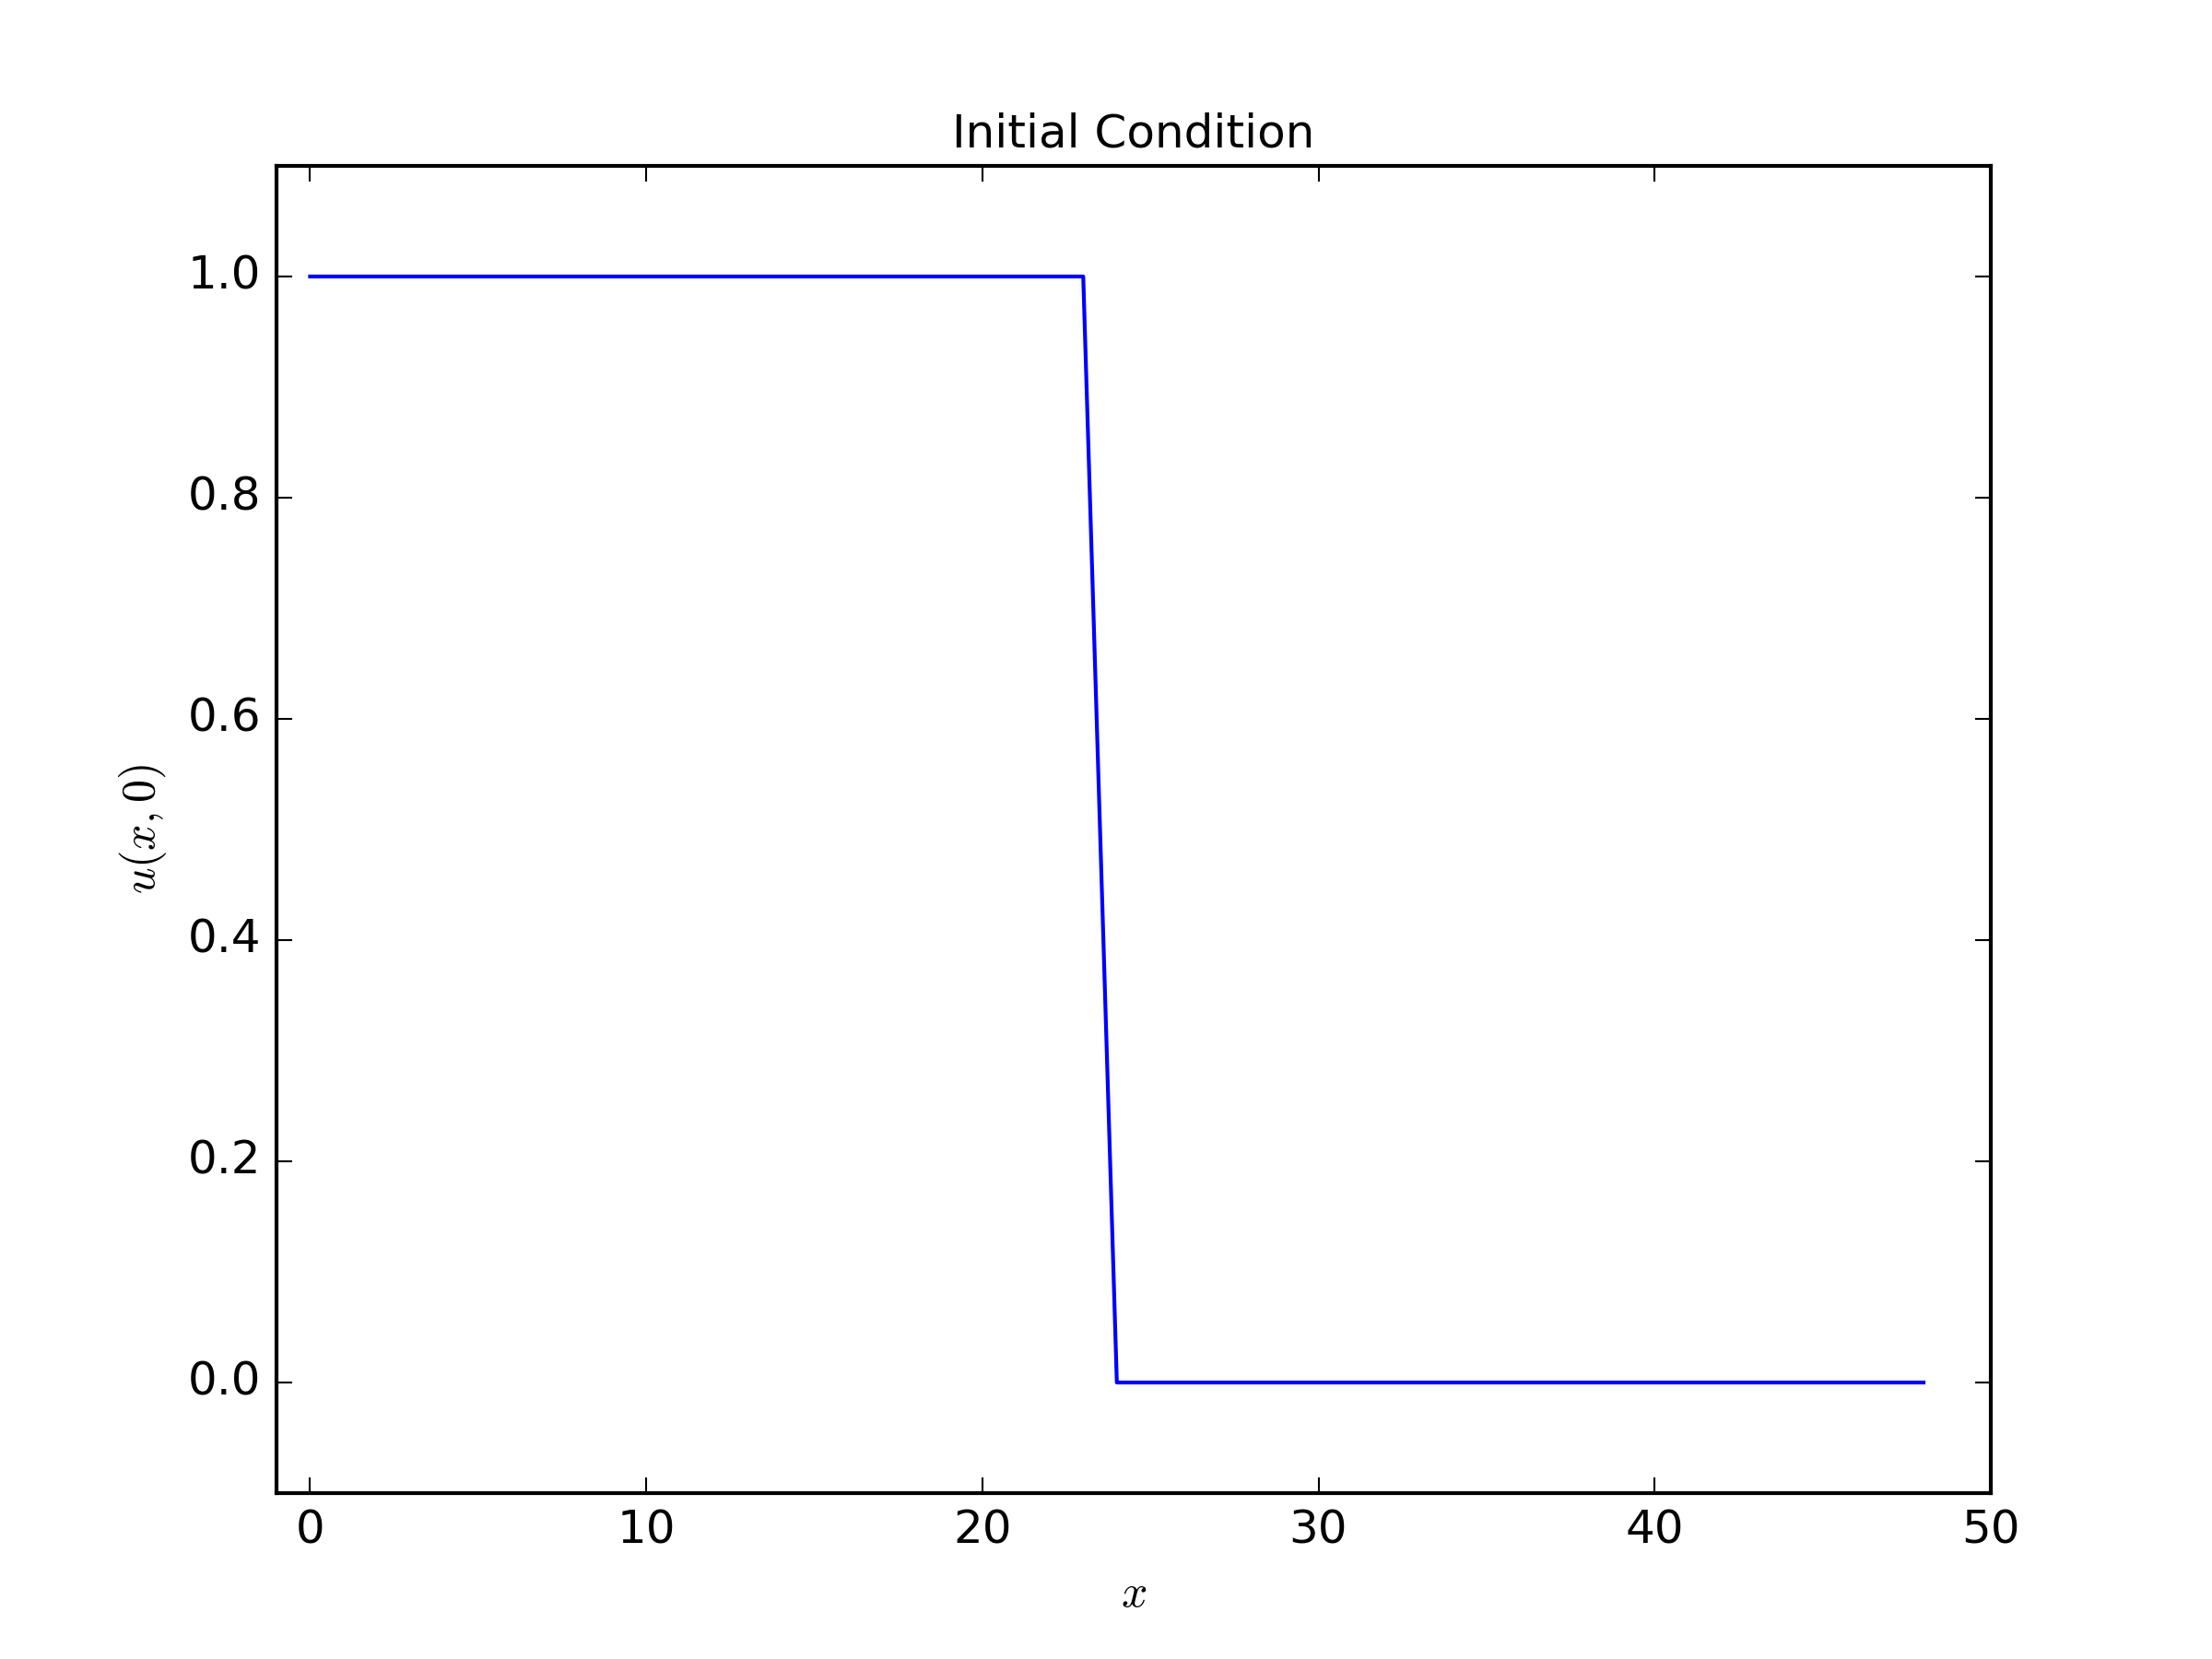
\includegraphics[width=0.75\textwidth]{problem3_initial_condition.png}
\end{figure}

With Crank-Nicolson with grid spacing $\Delta x = 0.02$ and time step $\Delta t = 0.1$, the solution at time $t=1$ develops a noisy disturbance about the discontinuity at $x=0.5$ from the initial condition.

\begin{figure}[H]
\centering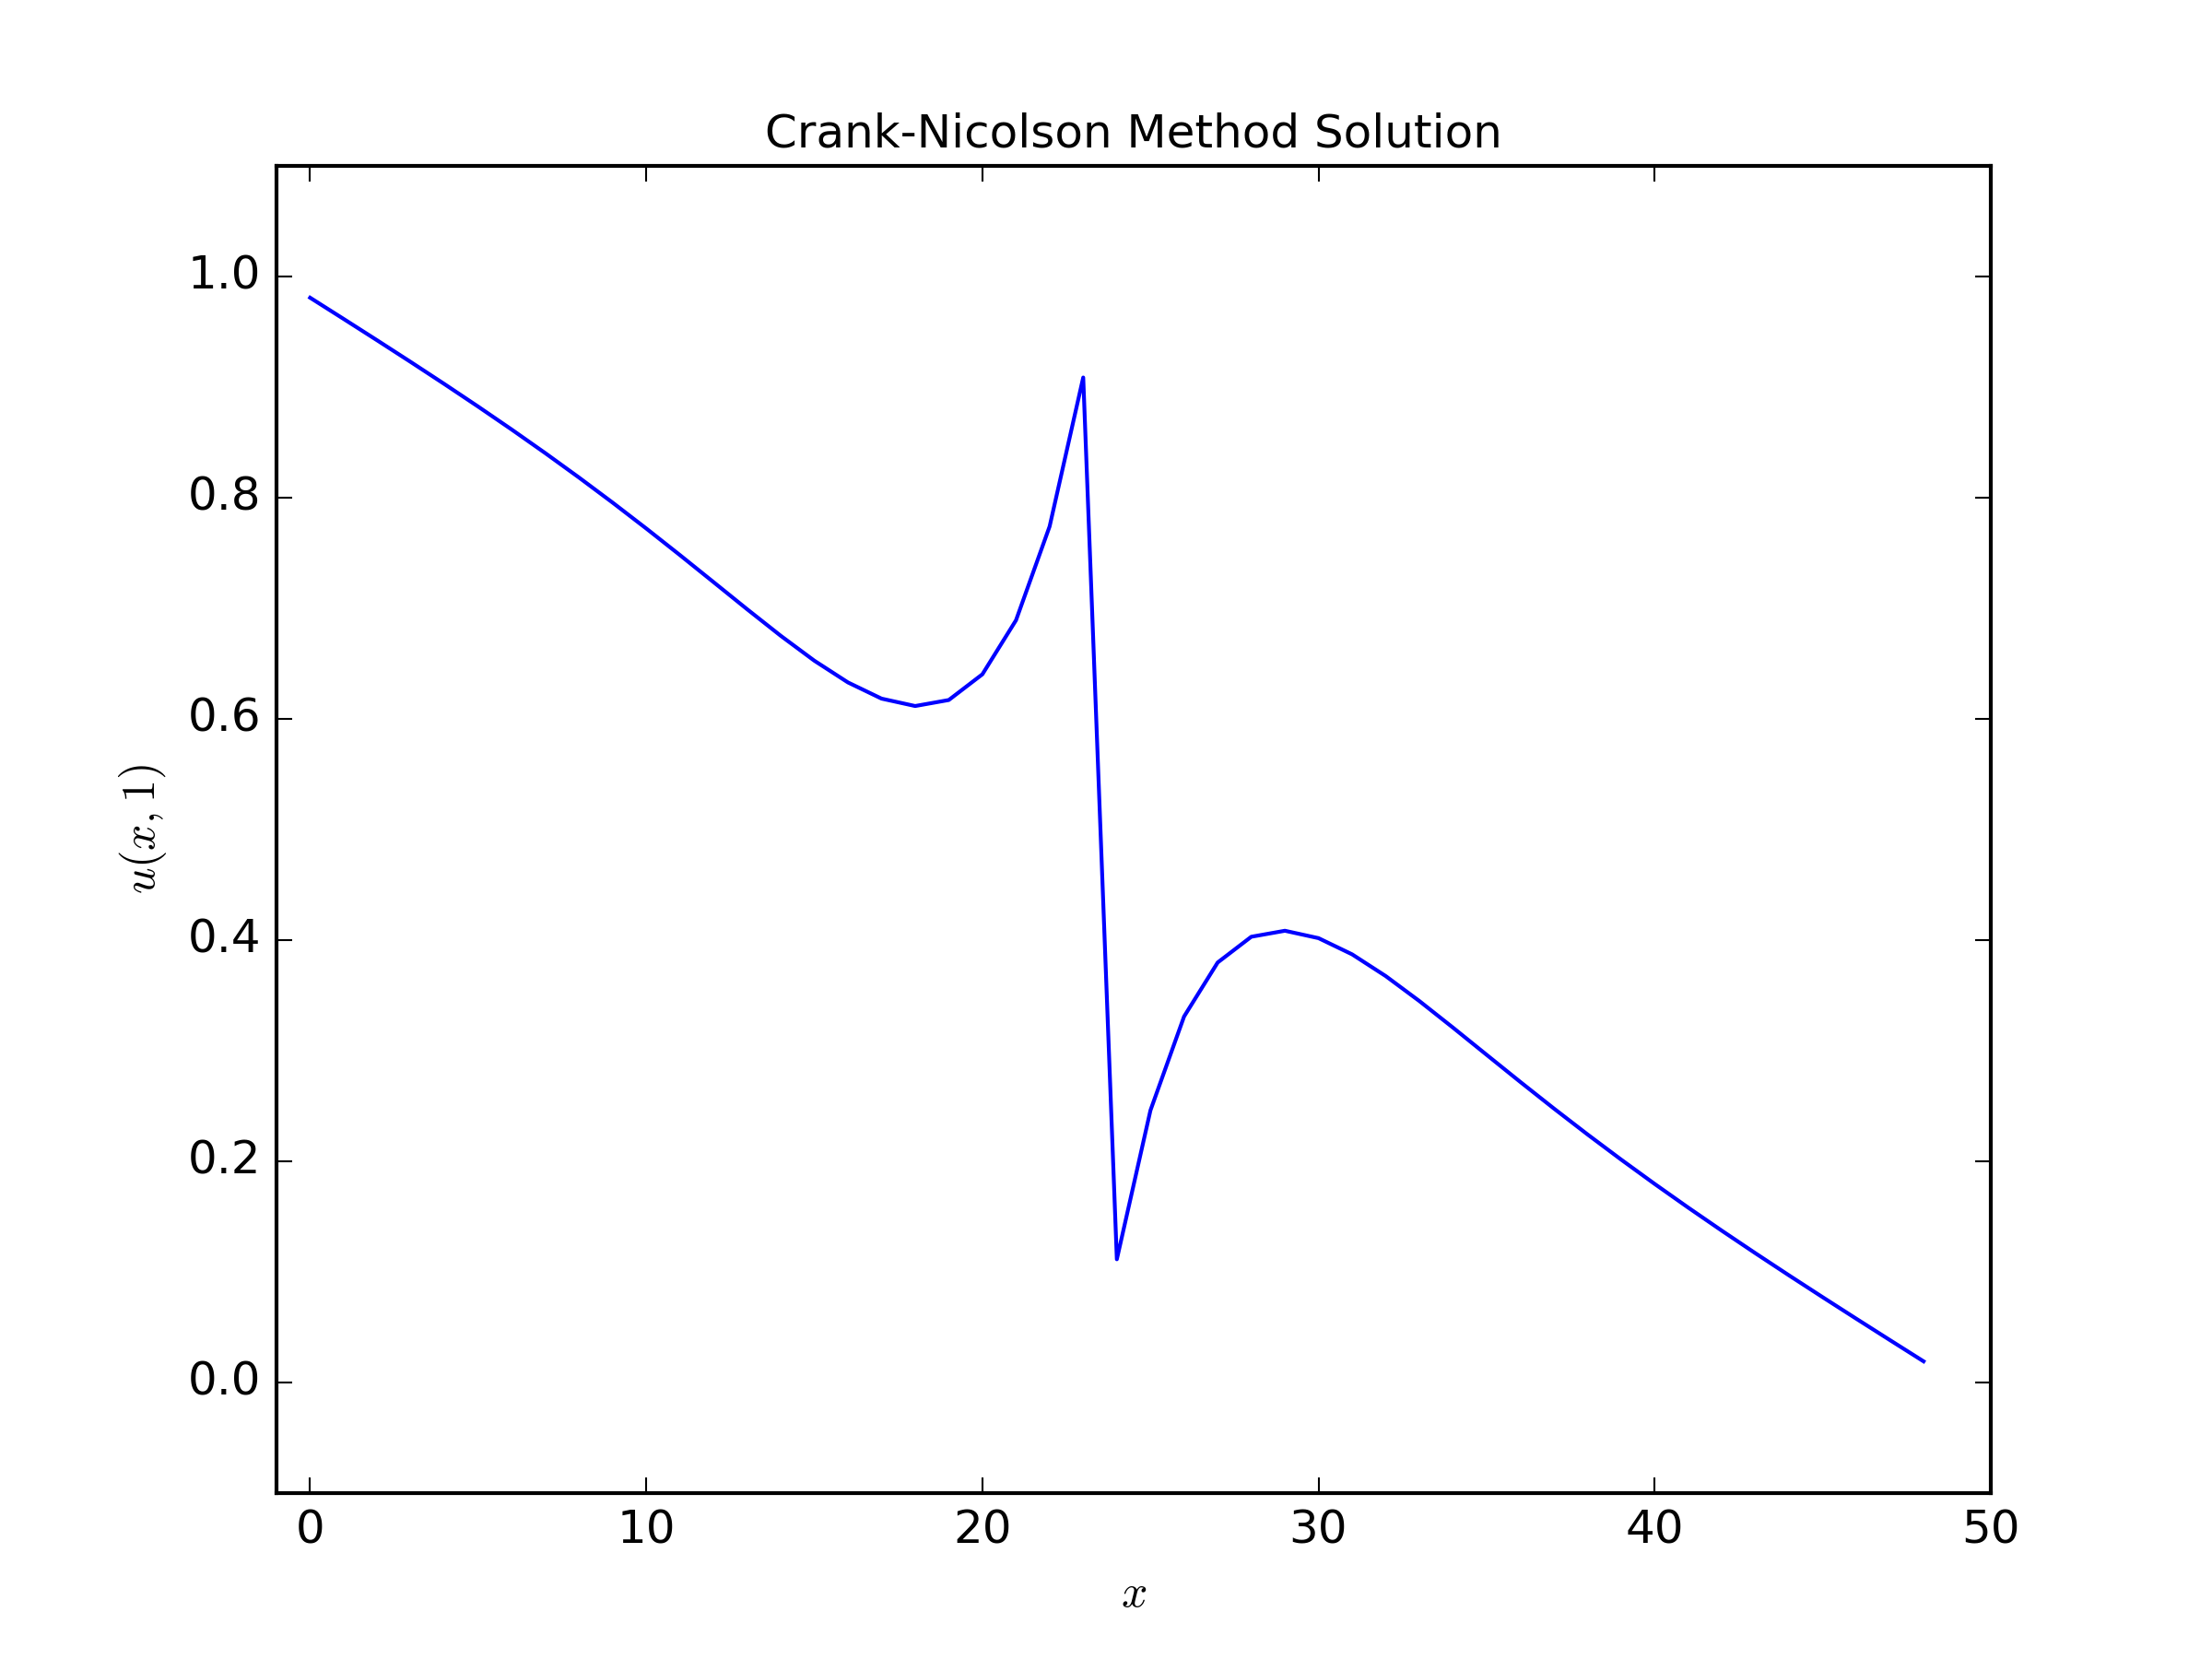
\includegraphics[width=0.75\textwidth]{problem3_crank_nicolson_issue.png}
\end{figure}

\item Give a mathematical argument to explain the unphysical behavior you observed in the numerical solution.

\item Repeat the simulation using BDF2, and discuss why the unphysical behavior is not present in the numerical solution for any time step.
\end{enumerate}

With BDF-2 and the same grid spacing $\Delta x = 0.02$, time step $\Delta t = 0.1$, the solution at time $t=1$ looks smooth and linear as it should.

\begin{figure}[H]
\centering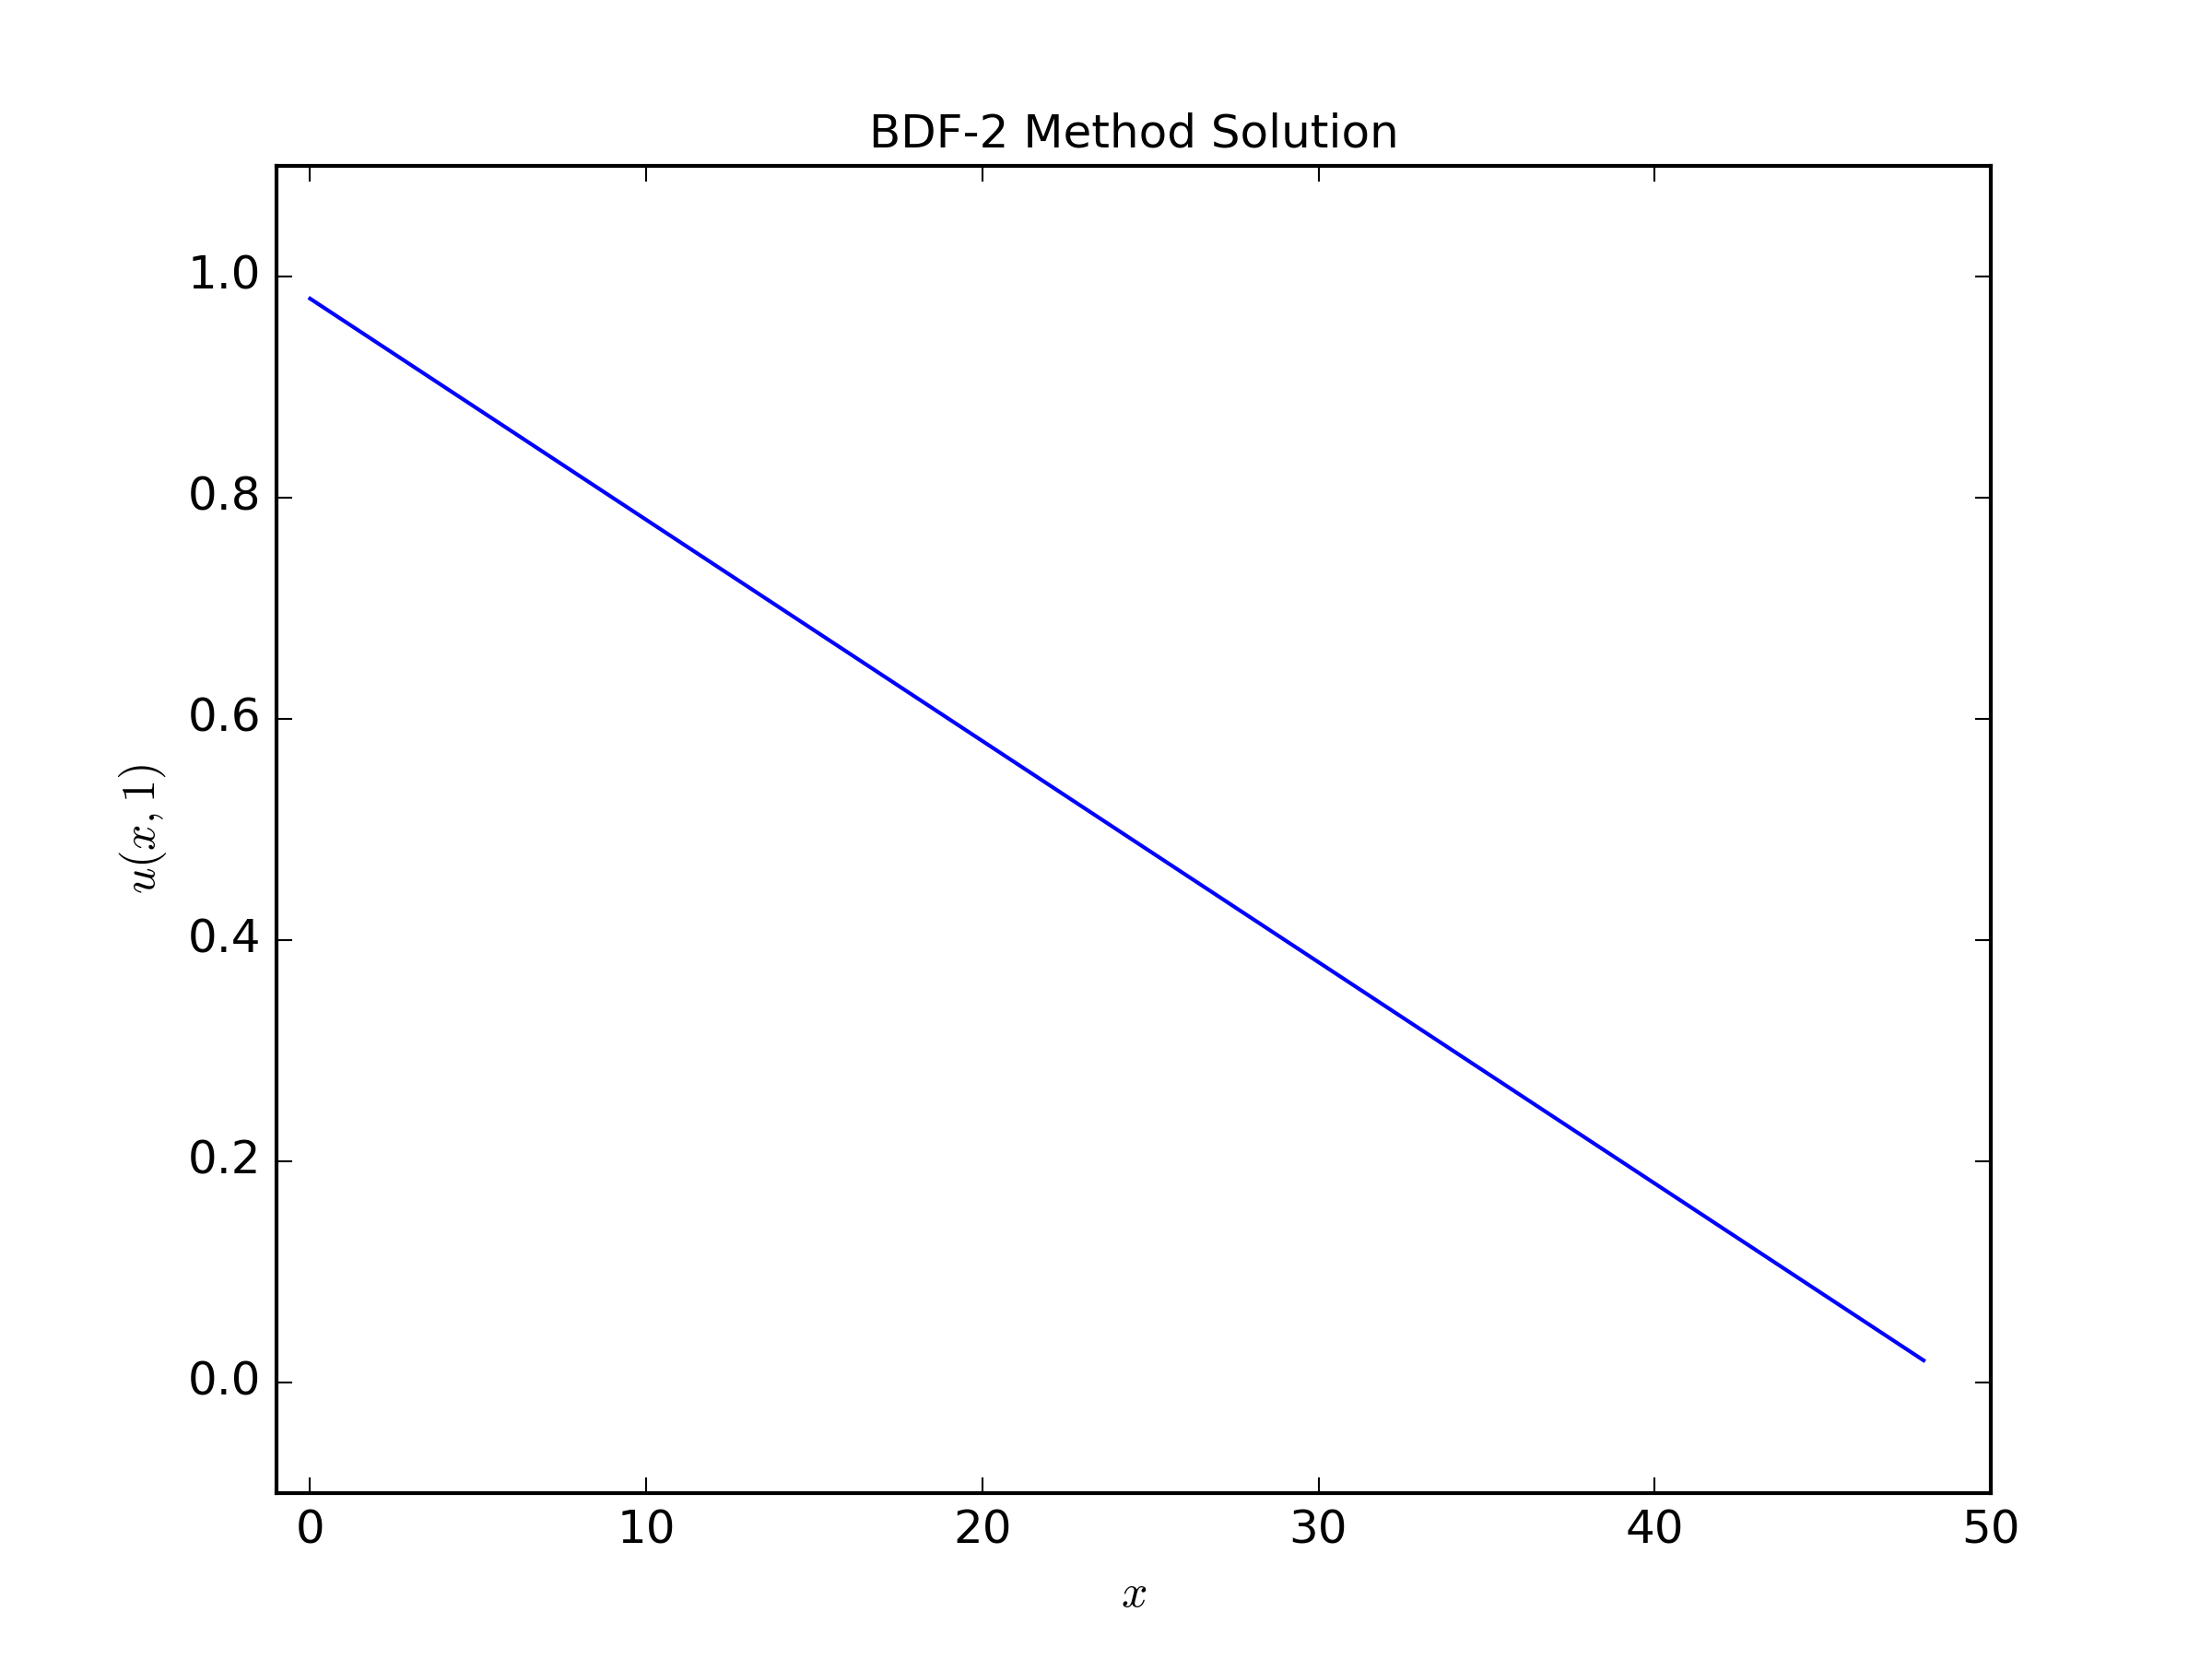
\includegraphics[width=0.75\textwidth]{problem3_bdf2_fixedissue.png}
\end{figure}

%%%%%%%%%%%%%%%%%%%%%%%%%%%%%%%%%%%%%%%%%%%%%%%%%%%%%%% CODE
The code used for the refinement study in Problem 2 is as follows:
\begin{verbatim}
#Refinement_study.py

from __future__ import division

import numpy as np
from numpy import exp, sin, pi
from numpy.linalg import norm
import matplotlib.pyplot as plt

from tabulate import tabulate
from tqdm import tqdm

from crank_nicolson import crank_nicolson_method
from bdf2 import bdf2_method

def succ_diff_refinement_study():
  #perform a refinement study to demonstrate Crank-Nicolson
  #is second-order accurate in space and time
  #using successive differences
  #since no analytic soln

  #max number of del_x,del_t values to examine
  refine_MAX = 10

  #loop through del_x values
  del_x = [2**(-2-i) for i in range(0,refine_MAX)]
  del_t = [2**(-1-i) for i in range(0, refine_MAX)]

  #set container for successive differences
  diffs = np.zeros(refine_MAX)

  #get u(x,1) through Crank-Nicolson:
  u_new = run_problem(del_x[0], del_t[0])

  #loop over finer del_x, take successive differences
  for i in tqdm(range(1,refine_MAX)):
    #store previous iterate
    u_old = u_new + 0

    #get next u(x,1) through Crank-Nicolson
    u_new = run_problem(del_x[i], del_t[i])
    
    #calculate successive difference between u(x,1) new and old 
    diffs[i] = del_x[i-1]*norm(restriction(u_new, del_x[i]) - u_old,1)

  #tabulate refinement study results
  two_norm_table = [[del_x[i], del_t[i], diffs[i], diffs[i]/diffs[i+1]] for i in range(refine_MAX-1)] 
  print(tabulate(two_norm_table, headers=['delta x', 'delta t', 'diffs', 'diff ratios'], tablefmt="latex"))

def errors_refinement_study():
  #perform a refinement study to demonstrate Crank-Nicolson
  #is second-order accurate in space and time
  #using error analysis with known analytic soln

  #max number of del_x,del_t values to examine
  refine_MAX = 10

  #loop through del_x values
  del_x = [2**(-2-i) for i in range(0,refine_MAX)]
  del_t = [2**(-1-i) for i in range(0, refine_MAX)]

  #set container for successive differences
  errors = np.zeros(refine_MAX)

  #loop over finer del_x and del_t
  for i in tqdm(range(0,refine_MAX)):
    #get approx u(x,1) through Crank-Nicolson
    [u_approx, u_sol] = run_test(del_x[i], del_t[i])
    
    #calculate error between u(x,1) approx and known solution 
    errors[i] = del_x[i]*norm(u_approx - u_sol,1)

  #tabulate refinement study results
  two_norm_table = [[del_x[i], del_t[i], errors[i], errors[i]/errors[i+1]] for i in range(refine_MAX-1)]  
  print(tabulate(two_norm_table, headers=['delta x', 'delta t', 'errors', 'error ratios'], tablefmt="latex"))

def restriction(u_f, h):
  #simple restriction operation
  h2 = 2*h
  n2 = int(1/h2)-1
  u_c = np.zeros(n2, dtype=float)

  #loop over coarse mesh
  for i in range(0,n2):
    u_c[i] = u_f[2*i+1]
    
  return u_c

def run_test(del_x, del_t):
  #set up the vectors and parameters for Crank-Nicolson method and run
  #using diffusion coefficient, initial condition of test problem
  #u_t = u_xx
  #u(0,t)=u(1,t)=0
  #u(x,0)=sin(pi x)
  #which has solution u(x,t)=e^{-pi^2 t}sin(pi x)

  #make vector of forcing function at all times 
  Nx = int(1/del_x)-1
  Nt = int(1/del_t)
  x = [i*del_x for i in range(1, Nx+1)]
  t = [i*del_t for i in range(Nt+1)]
  
  #f = 0
  f = [0*t for t in t]
  
  #initial condition u(x,0)=sin(pi x)
  u = [sin(pi*x) for x in x]

  #known solution u(x,t)=e^{-pi^2(0.01)t}sin(pi x) at t=1:
  u_sol = [exp(-pi**2)*sin(pi*x) for x in x]

  #diffusion coefficient
  D = 1
  u = crank_nicolson_method(del_x, del_t, u, f, D)
  return u, u_sol 

def run_problem(del_x, del_t):
  #set up the vectors and parameters for Crank-Nicolson method and run
  #using diffusion coefficient, initial condition, forcing function from problem 2

  #make vector of forcing function at all times 
  Nx = int(1/del_x)-1
  Nt = int(1/del_t)
  # x = [i*del_x for i in range(0, Nx+1)]
  t = [i*del_t for i in range(0, Nt+1)]
  
  #f = 1-exp(-t)
  neg_t = [-t for t in t] 
  f = 1-exp(neg_t)
  
  #initial condition u(x,0)=0
  u = np.zeros(Nx)

  #diffusion coefficient
  D = 0.01
  u = crank_nicolson_method(del_x, del_t, u, f, D)
  return u  

if __name__ == '__main__':
  errors_refinement_study()
  succ_diff_refinement_study()

#Crank-Nicolson.py

from __future__ import division

import numpy as np

import scipy.sparse as sparse
import scipy.sparse.linalg

def sparse_matrices(del_x):
  #set sparse matrix L, the discrete Laplacian
  #for 3-pt 2nd order approximation

  #Set number of grid points
  N = 1/del_x - 1

  #set off-diagonal Laplacian components
  offdiag = (1/(del_x**2))*np.ones(N)
  #set diagonal Laplacian components
  diag = np.ones(N)*(-2/(del_x**2))

  #put diagonals together into sparse matrix format
  data = np.vstack((offdiag, diag,offdiag))
  L = sparse.dia_matrix((data, [-1, 0,1]), shape = (N,N))

  #create identity matrix of same size as L
  I = sparse.identity(N)

  return L, I

def crank_nicolson_time_step(del_t, u, L, f, I):
  #one time step of crank-nicolson solver

  #(I + del_t/2 L)u^n
  A = (I + (del_t/2) * L)
  RHS_terms = A.dot(u) + del_t*f

  #make LHS matrix, put in CSC form for solver
  LHS_matrix = scipy.sparse.csc_matrix(I-(del_t/2)*L)

  #solve (I-del_t/2 L)u^n+1 = (I + del_t/2 L)u^n + del_t f^n+1/2
  u_next = scipy.sparse.linalg.spsolve(LHS_matrix, RHS_terms)

  return u_next

def crank_nicolson_method(del_x, del_t, u, f, D):

  #create sparse matrices for crank-nicolson method
  [L, I] = sparse_matrices(del_x)

  #calculate number of time points after 0 up to 1 (inclusive)
  Nt = int(1/del_t)

  for t in range(0,Nt):
    #take half point of f for solve
    f_half = (f[t]+f[t+1])/2
    #solve for next u
    u = crank_nicolson_time_step(del_t, u, D*L, f_half, I)
    
  return u
\end{verbatim}
\end{document}